\section{Exploración Bivariada}\label{bivariada}


Según el Programa de las Naciones Unidas para el Desarrollo (PNUD) Colombia ha mejorado el índice de desarrollo humano por los logros en la cobertura de educación y salud e incrementar el ingreso per cápita. Esto permitió pasar del puesto 77 al 69. Sin embargo, preocupa estar de undécimo entre los países con peor distribución del ingreso; el ingreso de un rico equivale a lo que reciben 58 personas más pobres de Colombia, mientras en Dinamarca y Japón equivale a 24.7 y 24.9 respectivamente.

Una de las mayores barreras para reducir la pobreza es la inequidad distributiva de la riqueza. La sociedad colombiana es pobre, presenta una distribución desigual del ingreso y crece poco. Es probable que una mejor distribución del ingreso facilite el crecimiento económico, que sólo es posible con una base institucional confiable y con políticas macroeconómicas estables enfocadas hacia el desarrollo individual.


\begin{figure}[h]
\begin{Schunk}
\begin{Soutput}
       cabeLog  restoLog
[1,] 0.4873974 0.1773112
\end{Soutput}
\begin{Soutput}
         cabeLog restoLog
cabeLog  "1"     ""      
restoLog "0.84"  "1"     
\end{Soutput}
\end{Schunk}
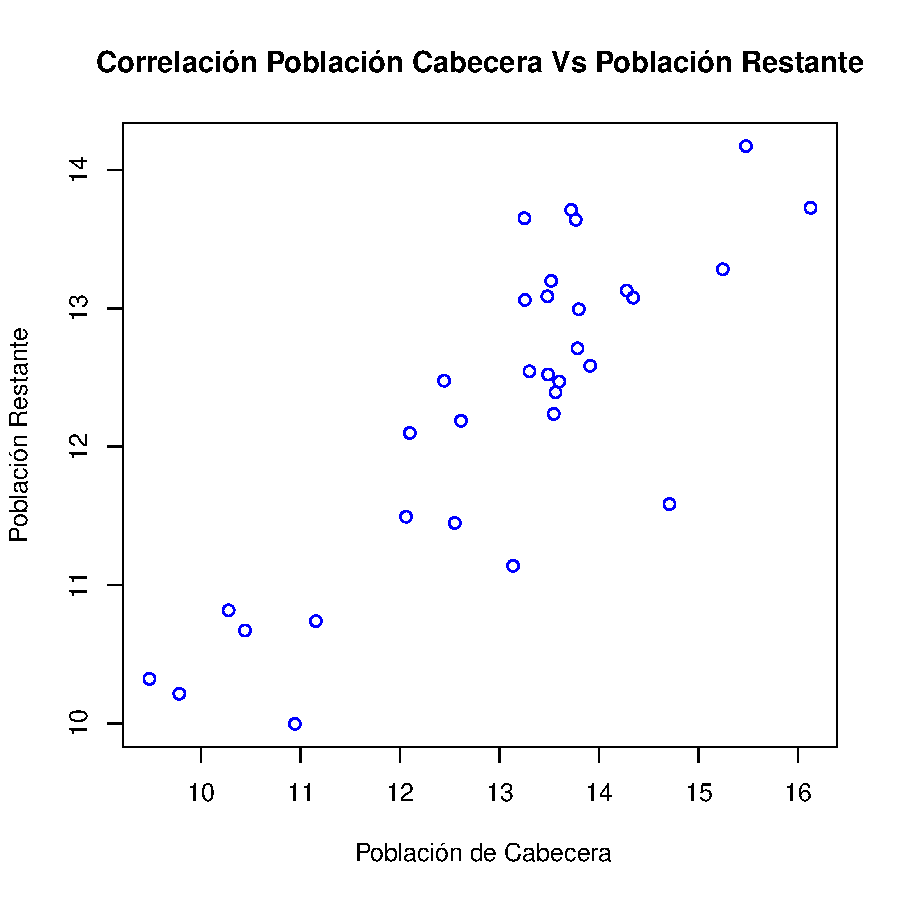
\includegraphics{bivariada-correl}
\end{figure}

\endinput
